\documentclass{standalone}
\usepackage{tikz}
\usetikzlibrary{patterns, positioning}

\begin{document}
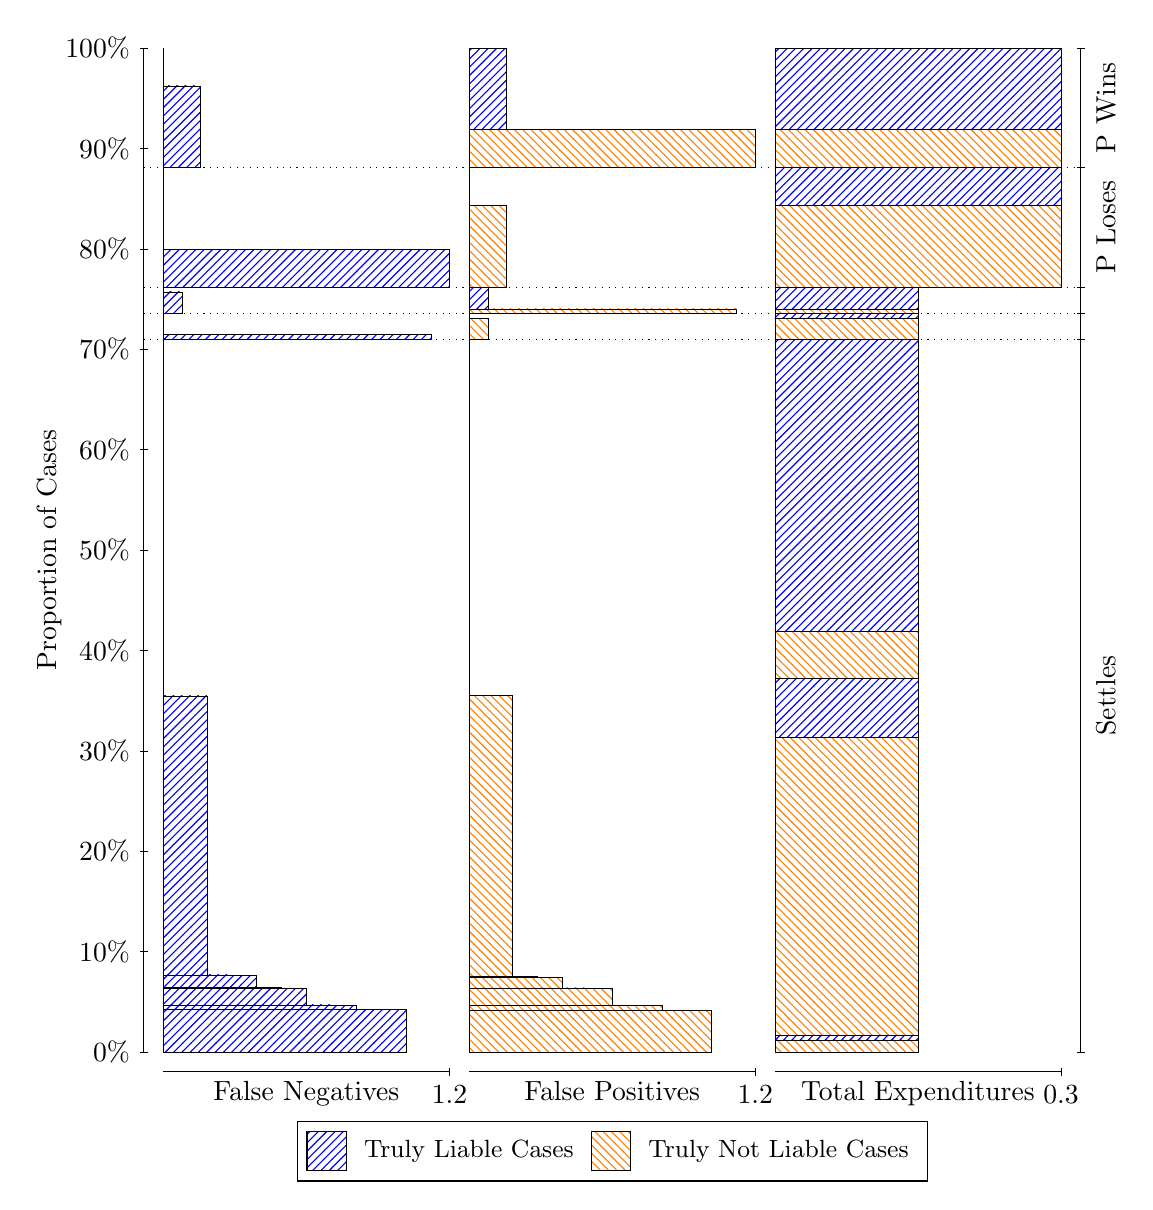
\begin{tikzpicture}
\draw[black, very thin] (1.5,1.75) -- (1.5,14.5);
\node[rotate=90, anchor=center] at (0.3, 8.125) {Proportion of Cases};
\draw[black, very thin] (1.45,1.75) -- (1.55,1.75);
\node[anchor=east] at (1.45, 1.75) {0\%};
\draw[black, very thin] (1.45,3.025) -- (1.55,3.025);
\node[anchor=east] at (1.45, 3.025) {10\%};
\draw[black, very thin] (1.45,4.3) -- (1.55,4.3);
\node[anchor=east] at (1.45, 4.3) {20\%};
\draw[black, very thin] (1.45,5.575) -- (1.55,5.575);
\node[anchor=east] at (1.45, 5.575) {30\%};
\draw[black, very thin] (1.45,6.85) -- (1.55,6.85);
\node[anchor=east] at (1.45, 6.85) {40\%};
\draw[black, very thin] (1.45,8.125) -- (1.55,8.125);
\node[anchor=east] at (1.45, 8.125) {50\%};
\draw[black, very thin] (1.45,9.4) -- (1.55,9.4);
\node[anchor=east] at (1.45, 9.4) {60\%};
\draw[black, very thin] (1.45,10.675) -- (1.55,10.675);
\node[anchor=east] at (1.45, 10.675) {70\%};
\draw[black, very thin] (1.45,11.95) -- (1.55,11.95);
\node[anchor=east] at (1.45, 11.95) {80\%};
\draw[black, very thin] (1.45,13.225) -- (1.55,13.225);
\node[anchor=east] at (1.45, 13.225) {90\%};
\draw[black, very thin] (1.45,14.5) -- (1.55,14.5);
\node[anchor=east] at (1.45, 14.5) {100\%};

\draw[black, very thin] (13.4,1.75) -- (13.4,14.5);
\draw[black, very thin] (13.35,1.75) -- (13.45,1.75);
\node[anchor=west] at (13.35, 1.75) {};
\draw[black, very thin] (13.35,10.802) -- (13.45,10.802);
\node[anchor=west] at (13.35, 10.802) {};
\draw[black, very thin] (13.35,11.128) -- (13.45,11.128);
\node[anchor=west] at (13.35, 11.128) {};
\draw[black, very thin] (13.35,11.464) -- (13.45,11.464);
\node[anchor=west] at (13.35, 11.464) {};
\draw[black, very thin] (13.35,12.982) -- (13.45,12.982);
\node[anchor=west] at (13.35, 12.982) {};
\draw[black, very thin] (13.35,14.5) -- (13.45,14.5);
\node[anchor=west] at (13.35, 14.5) {};

\draw[black, very thin, pattern color=blue, pattern=north east lines] (1.75,1.75) rectangle (4.8304,2.2863);
\draw[black, very thin, pattern color=blue, pattern=north east lines] (1.75,2.2863) rectangle (4.5145,2.2917);
\draw[black, very thin, pattern color=blue, pattern=north east lines] (1.75,2.2917) rectangle (4.1986,2.3413);
\draw[black, very thin, pattern color=blue, pattern=north east lines] (1.75,2.3413) rectangle (3.8826,2.3484);
\draw[black, very thin, pattern color=blue, pattern=north east lines] (1.75,2.3484) rectangle (3.5667,2.5585);
\draw[black, very thin, pattern color=blue, pattern=north east lines] (1.75,2.5585) rectangle (3.2507,2.5686);
\draw[black, very thin, pattern color=blue, pattern=north east lines] (1.75,2.5686) rectangle (2.9348,2.7235);
\draw[black, very thin, pattern color=blue, pattern=north east lines] (1.75,2.7235) rectangle (2.6188,2.73);
\draw[black, very thin, pattern color=blue, pattern=north east lines] (1.75,2.73) rectangle (2.3029,6.2724);
\draw[black, very thin, pattern color=orange, pattern=north west lines] (1.75,6.2724) rectangle (1.75,10.802);
\draw[black, very thin, pattern color=blue, pattern=north east lines] (1.75,10.802) rectangle (5.1464,10.861);
\draw[black, very thin, pattern color=orange, pattern=north west lines] (1.75,10.861) rectangle (1.75,11.128);
\draw[black, very thin, pattern color=blue, pattern=north east lines] (1.75,11.128) rectangle (1.987,11.404);
\draw[black, very thin, pattern color=orange, pattern=north west lines] (1.75,11.404) rectangle (1.75,11.464);
\draw[black, very thin, pattern color=blue, pattern=north east lines] (1.75,11.464) rectangle (5.3833,11.944);
\draw[black, very thin, pattern color=orange, pattern=north west lines] (1.75,11.944) rectangle (1.75,12.982);
\draw[black, very thin, pattern color=blue, pattern=north east lines] (1.75,12.982) rectangle (2.2239,14.02);
\draw[black, very thin, pattern color=orange, pattern=north west lines] (1.75,14.02) rectangle (1.75,14.5);
\draw[black, very thin, pattern color=orange, pattern=north west lines] (5.6333,1.75) rectangle (8.7138,2.2776);
\draw[black, very thin, pattern color=orange, pattern=north west lines] (5.6333,2.2776) rectangle (8.3978,2.2828);
\draw[black, very thin, pattern color=orange, pattern=north west lines] (5.6333,2.2828) rectangle (8.0819,2.3387);
\draw[black, very thin, pattern color=orange, pattern=north west lines] (5.6333,2.3387) rectangle (7.7659,2.3456);
\draw[black, very thin, pattern color=orange, pattern=north west lines] (5.6333,2.3456) rectangle (7.45,2.5552);
\draw[black, very thin, pattern color=orange, pattern=north west lines] (5.6333,2.5552) rectangle (7.1341,2.5582);
\draw[black, very thin, pattern color=orange, pattern=north west lines] (5.6333,2.5582) rectangle (7.1341,2.5651);
\draw[black, very thin, pattern color=orange, pattern=north west lines] (5.6333,2.5651) rectangle (6.8181,2.7011);
\draw[black, very thin, pattern color=orange, pattern=north west lines] (5.6333,2.7011) rectangle (6.5022,2.7077);
\draw[black, very thin, pattern color=orange, pattern=north west lines] (5.6333,2.7077) rectangle (6.1862,6.2797);
\draw[black, very thin, pattern color=blue, pattern=north east lines] (5.6333,6.2797) rectangle (5.6333,10.802);
\draw[black, very thin, pattern color=orange, pattern=north west lines] (5.6333,10.802) rectangle (5.8703,11.069);
\draw[black, very thin, pattern color=blue, pattern=north east lines] (5.6333,11.069) rectangle (5.6333,11.128);
\draw[black, very thin, pattern color=orange, pattern=north west lines] (5.6333,11.128) rectangle (9.0297,11.188);
\draw[black, very thin, pattern color=blue, pattern=north east lines] (5.6333,11.188) rectangle (5.8703,11.464);
\draw[black, very thin, pattern color=orange, pattern=north west lines] (5.6333,11.464) rectangle (6.1072,12.502);
\draw[black, very thin, pattern color=blue, pattern=north east lines] (5.6333,12.502) rectangle (5.6333,12.982);
\draw[black, very thin, pattern color=orange, pattern=north west lines] (5.6333,12.982) rectangle (9.2667,13.462);
\draw[black, very thin, pattern color=blue, pattern=north east lines] (5.6333,13.462) rectangle (6.1072,14.5);
\draw[black, very thin, pattern color=orange, pattern=north west lines] (9.5167,1.75) rectangle (11.333,1.9025);
\draw[black, very thin, pattern color=blue, pattern=north east lines] (9.5167,1.9025) rectangle (11.333,1.9646);
\draw[black, very thin, pattern color=orange, pattern=north west lines] (9.5167,1.9646) rectangle (11.333,5.7462);
\draw[black, very thin, pattern color=blue, pattern=north east lines] (9.5167,5.7462) rectangle (11.333,6.4925);
\draw[black, very thin, pattern color=orange, pattern=north west lines] (9.5167,6.4925) rectangle (11.333,7.0882);
\draw[black, very thin, pattern color=blue, pattern=north east lines] (9.5167,7.0882) rectangle (11.333,10.802);
\draw[black, very thin, pattern color=orange, pattern=north west lines] (9.5167,10.802) rectangle (11.333,11.069);
\draw[black, very thin, pattern color=blue, pattern=north east lines] (9.5167,11.069) rectangle (11.333,11.128);
\draw[black, very thin, pattern color=orange, pattern=north west lines] (9.5167,11.128) rectangle (11.333,11.188);
\draw[black, very thin, pattern color=blue, pattern=north east lines] (9.5167,11.188) rectangle (11.333,11.464);
\draw[black, very thin, pattern color=orange, pattern=north west lines] (9.5167,11.464) rectangle (13.15,12.502);
\draw[black, very thin, pattern color=blue, pattern=north east lines] (9.5167,12.502) rectangle (13.15,12.982);
\draw[black, very thin, pattern color=orange, pattern=north west lines] (9.5167,12.982) rectangle (13.15,13.462);
\draw[black, very thin, pattern color=blue, pattern=north east lines] (9.5167,13.462) rectangle (13.15,14.5);
\draw[black, dotted] (1.5,10.802) -- (13.4,10.802);
\draw[black, dotted] (1.5,11.128) -- (13.4,11.128);
\draw[black, dotted] (1.5,11.464) -- (13.4,11.464);
\draw[black, dotted] (1.5,12.982) -- (13.4,12.982);
\draw[black, very thin] (1.75,1.5) -- (5.3833,1.5);
\node[anchor=north] at (3.5667, 1.5) {False Negatives};
\draw[black, very thin] (5.3833,1.45) -- (5.3833,1.55);
\node[anchor=north] at (5.3833, 1.45) {1.2};

\draw[black, very thin] (5.6333,1.5) -- (9.2667,1.5);
\node[anchor=north] at (7.45, 1.5) {False Positives};
\draw[black, very thin] (9.2667,1.45) -- (9.2667,1.55);
\node[anchor=north] at (9.2667, 1.45) {1.2};

\draw[black, very thin] (9.5167,1.5) -- (13.15,1.5);
\node[anchor=north] at (11.333, 1.5) {Total Expenditures};
\draw[black, very thin] (13.15,1.45) -- (13.15,1.55);
\node[anchor=north] at (13.15, 1.45) {0.3};

\node[black, centered, rotate=90] at (13.72, 6.2761) {Settles};


\node[black, centered, rotate=90] at (13.72, 12.223) {P Loses};
\node[black, centered, rotate=90] at (13.72, 13.741) {P Wins};

\draw (7.449999999999999,1.5) node[draw=none] (baseCoordinate) {};
\begin{scope}[align=center]
        \matrix[scale=0.5, draw=black, below=0.5cm of baseCoordinate, nodes={draw}, column sep=0.1cm]{
            \node[rectangle, draw, minimum width=0.5cm, minimum height=0.5cm, pattern=north east lines, pattern color=blue] {}; &
            \node[draw=none, font=\small] (B) {Truly Liable Cases}; &
            \node[rectangle, draw, minimum width=0.5cm, minimum height=0.5cm, pattern=north west lines, pattern color=orange] {}; &
            \node[draw=none, font=\small] (B) {Truly Not Liable Cases}; \\
            };
\end{scope}

\end{tikzpicture}
\end{document}